\section{Resultados}
% Se muestran e interpretan los resultados como se obtuvieron

Empecemos describiendo los parámetros del problema los cuales son:
\begin{itemize}
    \item \textbf{Número de paquetes:} 1000
    \item \textbf{Capacidad Máxima de cada contenedor:} 36
    \item \textbf{Capacidad Máxima de cada columna:} 12
    \item \textbf{Mín columnas necesarias:} 401
\end{itemize}

Al ejecutar nuestro algoritmo de colonia de hormigas para el problema de bin packing con los datos generados, considerando 20 hormigas y 100 iteraciones,
obtuvimos los siguientes resultados:

\begin{itemize}
    \item \textbf{Tamaño Total de paquetes:} 4802
    \item \textbf{Columnas usadas en ACO:} 483 (aproximadamente 20\% más que el mínimo por el factor de holgura)
    \item \textbf{Capacidad Máxima total:} 5796
    \item \textbf{Mejor solución encontrada:} 161 contenedores utilizados.
    \item \textbf{Carga promedio de cada contenedor en la mejor solución:} 29.83
    \item \textbf{Carga promedio de cada columna en la mejor solución:} 11.27
\end{itemize}

Ademas de esto podemos ver la evolución del mejor fitness y el fitness promedio a lo largo de las iteraciones en la siguente figura:
\begin{figure}[H]
    \centering
    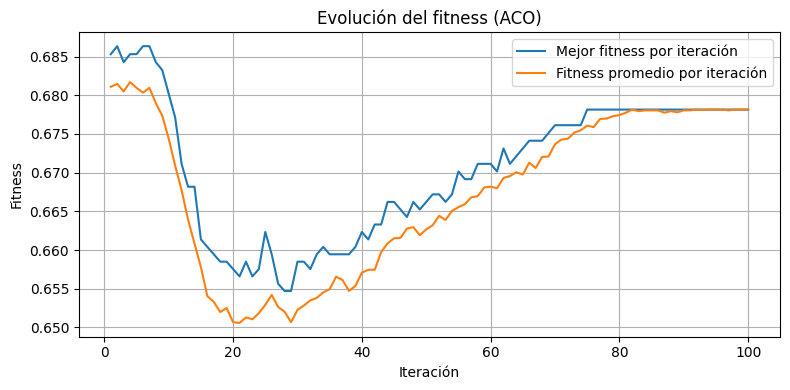
\includegraphics[width=1\textwidth]{rsc/img/des/fitness.png}
    \caption{Evolución del fitness a lo largo de las iteraciones}\label{fig:fitness}
\end{figure}

Cave resaltar el comportamiento del algoritmo donde se observa como el fitness promedio y el mejor decaen rápidamente en las primeras iteraciones, indicando
un proceso de exploración que decae debido a la evaporacion para despues empezar a estabilizarse conforme se acerca a una solución óptima ademas de que
al acercarse el promedio al mejor fitness indica que las soluciones generadas por las hormigas explotan cada vez más las mejores rutas de feromonas encontradas.

Finalmente para nuestro problema de bin packing vemos las siguentes graficas mostrando la capacidad utilizada en cada contenedor y columna respectivamente:
\begin{figure}[H]
    \centering
    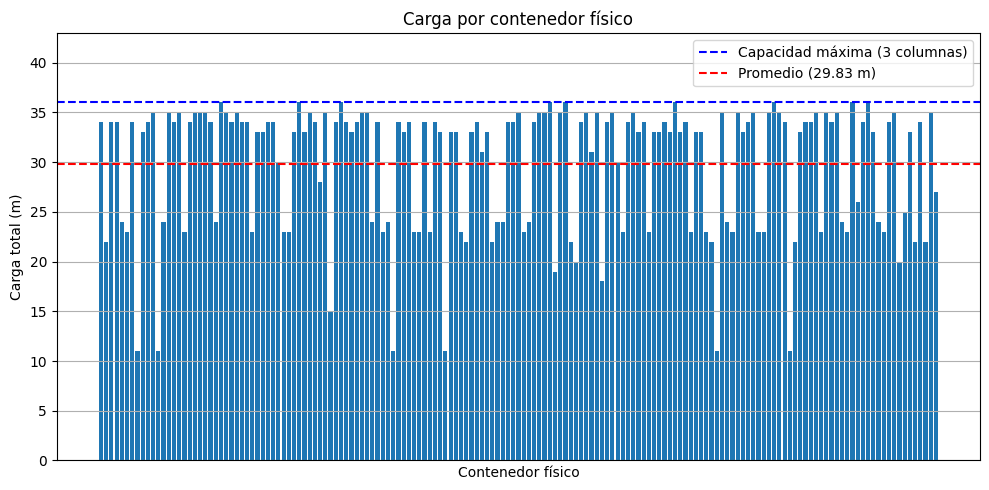
\includegraphics[width=1\textwidth]{rsc/img/des/carga_x_contenedor.png}
    \caption{Carga utilizada en cada contenedor en la mejor solución}\label{fig:xcont}
\end{figure}

\begin{figure}[H]
    \centering
    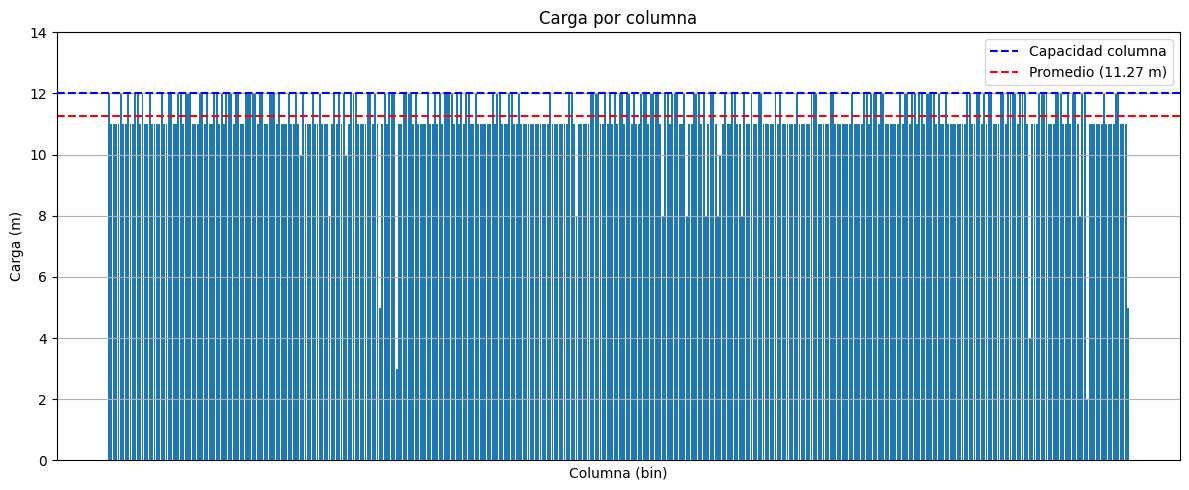
\includegraphics[width=1\textwidth]{rsc/img/des/carga_x_columna.png}
    \caption{Carga utilizada en cada columna en la mejor solución}\label{fig:xcol}
\end{figure}